\section{Introduction}
\ifrevision
\reversemarginpar
\marginpar{D3,F1}
\fi
Recent years have witnessed the widespread use of sophisticated frameworks, such as Hadoop MapReduce \cite{hadoop}, Dryad \cite{dryad}, Spark \cite{spark}, and Apache Tez \cite{tez}.
Most of them define jobs as directed acyclic graphs (DAGs), such as map-reduce pipeline in Hadoop MapReduce, lineage of resilient distributed datasets (RDDs) in Spark, vertices and edges in Dryad and Tez, etc.
Despite the differences among data-intensive frameworks, their communication is always structured as a shuffle phase,  which takes place between successive computation stages. 
Such shuffle phase places a significant burden for both the disk and network I/O, thus heavily affecting the end-to-end application performance. 
For instance, a MapReduce trace analysis from Facebook shows that shuffle accounts for 33\% of the job completion time on average, and up to 70\% in shuffle-heavy jobs \cite{managing}.

Although continuous efforts of performance optimization have been made among a variety of computing frameworks \cite{sync, babu, tachyon, pacman, quincy, delay}, 
the shuffle is often poorly optimized in practice.
% take over shuffle
%shuffle characteristic
In particular, we observe that one major deficiency lies in the lack of fine-grained, coordinated management among different system resources.
%In the current practice, the shuffle phase is often split into two parts --- \textit{shuffle read} and \textit{shuffle write}. 
As Figure \ref{fig:workflow} shows, the \textit{shuffle write} is responsible for writing intermediate results to disk, which is attached to the tasks in ancestor stages (i.e., map task).  
And the \textit{shuffle read} fetches intermediate results from remote disks through network, which is commonly integrated as part of the tasks in descendant stages (i.e., reduce task). 
Once scheduled, a fixed bundle of resources (i.e., CPU, memory, disk and network) named \textit{slot} is assigned a task, and the resources are released only after the task finishes.
\ifrevision
\marginpar{D2}
\fi
Such task aggregation together with the coarse-grained scheduling effectively simplifies task management.
However, since a cluster has a limited number of slots, attaching the I/O intensive shuffle phase to the CPU/memory intensive computation phase results in a poor multiplexing between computational and I/O resources.
%The map task in Figure \ref{fig:workflow} well explains such deficiency: the I/O resource allocated to the stage is always idle during the computation time, and the computation/memory resource is totally wasted during the shuffle write attached to it, and vice versa.
\begin{figure}
	\centering
	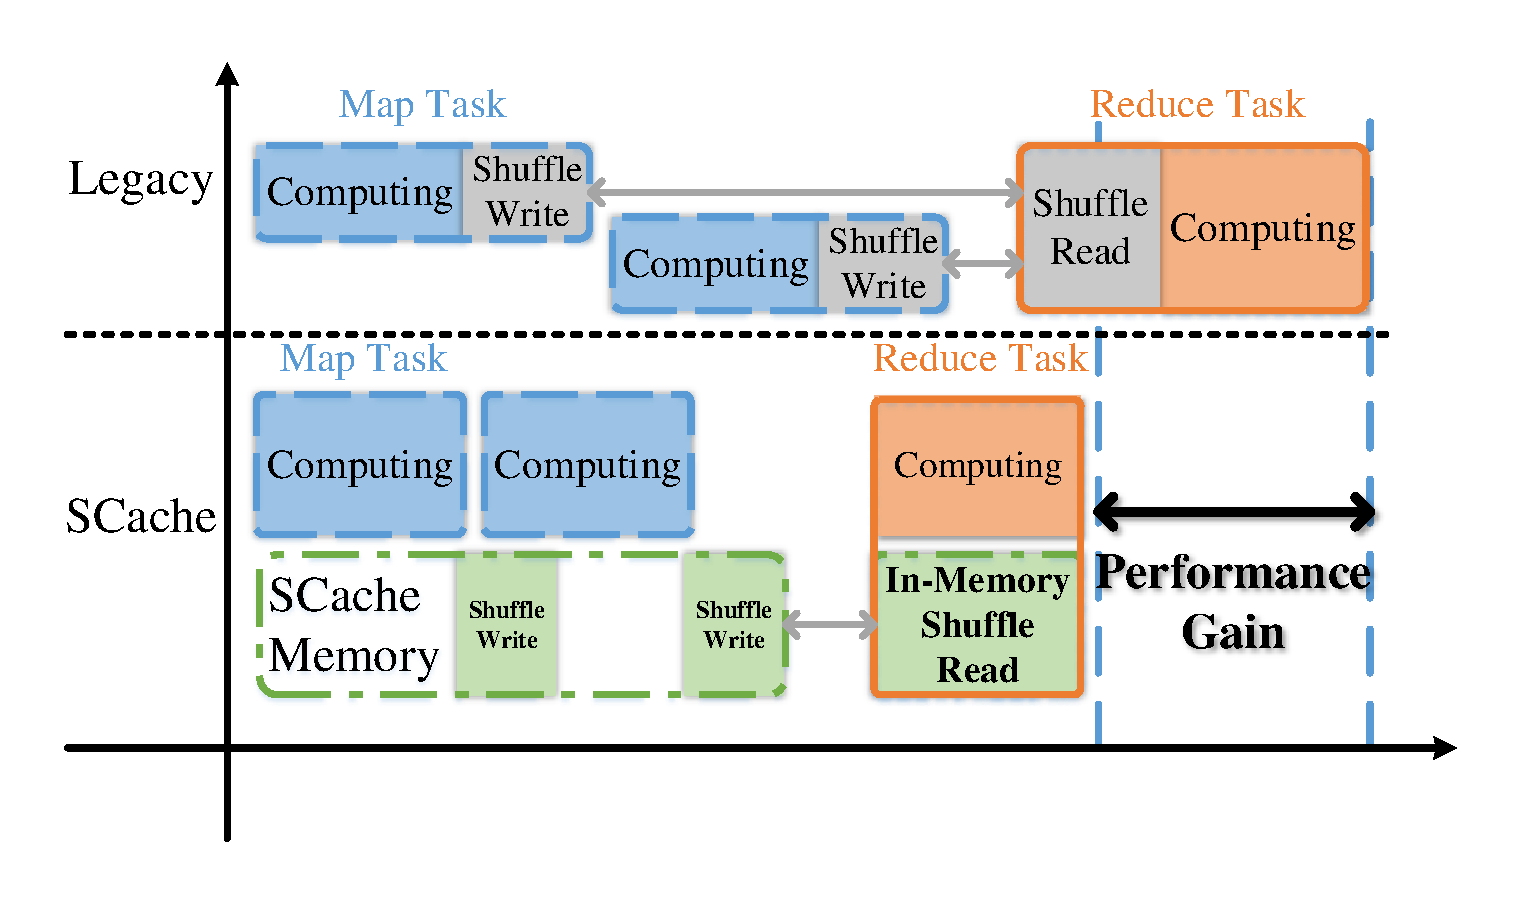
\includegraphics[width=\linewidth]{fig/workflow}
	\caption{Workflow Comparison between Legacy DAG Computing Frameworks and Frameworks with SCache}
	\label{fig:workflow}
	\vspace{-1.2em}
\end{figure}

Moreover, the shuffle read phase introduces all-to-all communication pattern across the network, and such network I/O procedure is also poorly coordinated.
Note that the shuffle read phase starts fetching data only after the corresponding reduce task starts.
Meanwhile, the reduce tasks belonging to a same execution phase are scheduled at the same time by default. 
As a result, all the corresponding reduce tasks start fetching shuffle data almost simultaneously.
Such synchronized network communication causes a burst demand for network I/O, which in turn greatly enlarges the shuffle read completion time. 
To desynchronize the network communication, an intuitive way is to launch some tasks in the descendent stage earlier, such as "slow-start" from Hadoop MapReduce\cite{hadoop}. 
However, such early-start is by no means a panacea. 
This is because the early-start always introduces an extra early allocation of the slot leading to a slow execution of the current stage.
% This is because although the reduce tasks can start fetching data earlier, the computation can only take place after all the data is ready. 

%In one word, existing solutions suffer from either inefficient use of network I/O, or a waste of computational resources (i.e., CPU and memory) caused by task pre-launching.

%For example, Apache Hadoop \cite{hadoop} provides an \emph{early start} mechanism that launches reduce tasks after a certain portion (5\% by default) of map tasks has completed, which is adopted in many of the recent works \cite{ihadoop, ishuffle, dynmr}.
% DAG computing framworks deriving from MapReduce \cite{mapreduce} contains a hard barrier between computing stages. The terminology of this barrier is \textit{shuffle}. Shuffle contains two parts on the connecting stages-\textit{shuffle write} and \textit{shuffle read}. On the side of ancestor stages, \textit{shuffle write} is resoponsible for writing intermediate results to disk. On the side of descendant stage, \textit{shuffle read} fetches intermediate results from remote disks through network. Although highly optimized in other factors, the shuffle of framework is still primitive.  The coarse design of shuffle introduce a significiant performance overhead.
% % design inconsistent
% For instance, a MapReduce trace analysis from Facebook shows that shuffle accounts for 33\% JCT on average, up to 70\% in shuffle-heavy jobs \cite{managing}.
% shuffle operations
% three resource coordinate 不好
% 计算和I/O couple, why
% why disk, reason!!!, 不重视
% common problems

To make things worse, we note that the above deficiencies generally exist in most of the DAG computing frameworks. 
As a result, even we can effectively resolve the above deficiencies by modifying one framework, updating one application at a time is impractical given the sheer number of computing frameworks available today.

% The main defect of current shuffle design is coarse granularity of resource allocation during the task scheduling.
% Nearly all task scheduling algorithms in DAG frameworks use time slotted model. Specifically, when a task is launched, the framework offers it a bundle of resources (i.e. CPU and memory), which are dedicated to this task during the time in its "slot".
% But for a task, the resources demand changes during different phases. The computing phase is CPU and memory intensive. The shuffle, instead, is I/O intensive.
% As shown in the upper part of Figure \ref{fig:workflow}, this "slot" can be released until the map tasks finish \textit{shuffle write} on disk. And the "slot" is occupied when the reduce tasks begin to read shuffle data from remote nodes through network, which is presented as \textit{shuffle read}. This inconsistency between demands and allocation results in a severe resource underutilization, which slow down the framework.

% Another drawback of current shuffle is the synchronized shuffle read. When all the reduce tasks are scheduled, the shuffle fetch of each task starts almost simultaneously, which may cause congestion of network and delay the shuffle read. The straight forward way to avoid network burst is to start reduce tasks earlier. Apache Hadoop \cite{hadoop} provides a mechanism that schedules reduce tasks when a certain portion of map tasks completed. So that the shuffle delay can be mitigated. Other publications also purpose solutions to pre-schedule reduce tasks \cite{ihadoop, ishuffle, dynmr}. However this early scheduling of reduce tasks occupies new task slots, which degrades system performance. To this end, we proposed a question for this cross-frameworks issue, \textit{can we efficiently optimize shuffle without manually change every DAG framework?}




% 针对性的提出这三个点
% three resource coordinate 不好
% 计算和I/O couple, why
% why disk, reason, 不重视
% common problems
% 总起:普适性工具
% pre-fetch but not pre-execute
% byproduct: more balance
% memory instead of disk

% challenge point by point, inside the problem

Can we efficiently optimize the data shuffling without significantly changing DAG frameworks?
In this paper, we answer this question in the affirmative with S(huffle)Cache, an open source \footnote{https://github.com/frankfzw/SCache} plug-in system which provides a shuffle-specific optimization for different DAG computing frameworks.
Specifically, SCache takes over the whole shuffle phase from the underlying framework by providing a cross-framework API for both shuffle write and read.
SCache's effectiveness lies in the following two key ideas.
First, SCache decouples the shuffle write and read from both map and reduce tasks.
\ifrevision
\marginpar{D2}
\fi
Such decoupling effectively enables fine-grained resource management and better multiplexing between the computational and I/O resources.
In addition, SCache pre-schedules the reduce tasks \emph{without launching} them and pre-fetches the shuffle data. 
% for the reduce tasks.
Such pre-scheduling and pre-fetching effectively overlap the network transfer time, desynchronize the network communication, 
and avoid the extra early allocation of slots.
%In this paper, we introduce S(huffle)Cache, an plugin system to remove shuffle latency for DAG frameworks. SCache takes over the management of shuffle and I/O resources to acheive a fine granularity scheduling of tasks. In addition, SCache pre-schedules the reduce tasks without launching them and perform shuffle data pre-fetch to break the synchronization of shuffle fetch. In order to provide a general optimization for different DAG frameworks, SCache decouple the shuffle process from computing and  provide a cross-frameworks API for shuffle write and read.

The workflow of a DAG framework with SCache is presented in Figure \ref{fig:workflow}. 
SCache replaces the disk operations of shuffle write by the memory copy in map tasks. 
The slot is released after the memory copy. 
The shuffle data is stored in the reserved memory of SCache until all reduce tasks are pre-scheduled. 
Then the shuffle data is pre-fetched according to the pre-scheduling results.  
The application-context-aware memory management caches the shuffle data in memory before launching the reduce task.
By applying these optimizations, SCache can help the DAG framework achieve a significant performance gain.  

The main challenge to achieve this optimization is \textit{pre-scheduling reduce tasks without launching}. 
% It is not critical for the simple DAG computing such as Hadoop MapReduce \cite{mapreduce}. 
First, the complexity of DAG can amplify the defects of na\"{i}ve scheduling schemes. 
In particular, randomly assigning reduce tasks might result in a collision of two heavy tasks on one node. 
This collision can aggravate data skew, thus hurting the performance. 
Second, pre-scheduling without launching violates the design of most frameworks that launch a task after scheduling.
To address the challenges, we propose a heuristic task pre-scheduling scheme with shuffle data prediction and a task co-scheduler (Section \ref{opt}).

Another challenge is the \textit{in-memory data management}. 
To prevent shuffle data touching the disk, SCache leverages extra memory to store the shuffle data. 
% However, the memory is a precious resource for DAG computing. 
To minimize the reserved memory while maximizing the performance gain, we propose two constraints: all-or-nothing and context-aware (Section \ref{memorymanage}).
%The memory management scheme follows these two contraints to switch shuffle data blocks on and off reserved memory.

We have implemented SCache and a customized Apache Spark \cite{apachespark}. 
The performance of SCache is evaluated with both simulations and testbed experiments on a 50-node Amazon EC2 cluster. 
We conduct basic test GroupByTest. 
We also evaluate the system with Terasort \cite{spark-tera} benchmark and standard workloads like TPC-DS \cite{tpcds} for multi-tenant modeling. 
In a nutshell, SCache can eliminate explicit shuffle process by at most $89\%$ in varied application scenarios. 
More impressively, SCache reduces $~40\%$ of overall completion time of TPC-DS queries on average.

